\documentclass[12pt,a4paper]{article}
\usepackage[portuges]{babel}
\usepackage[utf8]{inputenc}
\usepackage[T1]{fontenc}
\usepackage{amsmath}
\usepackage{amsfonts}
\usepackage{amssymb}
\usepackage{pgfplots}
\usepackage{filecontents}
\usepackage{cite}
\usepackage{subfigure}
\usepackage{tikz}
\usepackage{caption}
\usepackage{graphicx}
\usepackage{float}
\usepackage[lined,boxed,commentsnumbered]{algorithm2e}
\usepackage{rotating}

%%%%%%Information of the paper
\pdfinfo{
/Title (EP3 - Planejamento Heurístico)
/Author (Diego Araujo, Viviane Bonadia, Ignasi Andres)
}

%%%%%%%%Title
\title{MAC5788 - Relatório EP3: Planejamento Heurístico}
\author{Viviane Bonadia NUSP 9167607, Diego Ara\'{u}jo NUSP 7157092, \\ Ignasi Andr\'{e}s NUSP 8193481\\
Universidade de S\~{a}o Paulo\\
S\~{a}o Paulo, Brazil\\ \{vbonadia, diegoamc, ignasi\} @ime.usp.br}

\begin{document}
\maketitle

\section{Introdução}

%planejamento de busca heurística?
%planejamento de busca com heurística?
%planejamento heurístico de busca?
O planejamento de busca com heurística é uma técnica de planejamento que têm se mostrado eficiente na solução de problemas. Nela, uma função heurística é derivada a partir do problema e usada para guiar a busca na escolha dos próximos estados a serem explorados.
Neste trabalho apresentamos um planejador de busca heurística e avaliamos seu desempenho na solução de diferentes problemas de planejamento usando diversos parâmetros e heurísticas. 
Na seção \ref{planejamento} damos uma breve explicação de planejamento heurístico. Nas seções \ref{heuristicas} descrevemos as heurísticas implementadas no planejador e o algoritmo de busca usado para encontrar a solução de um dado problema. Utilizamos três problemas para análise do planejador: Problema dos Robôs, Mundo dos Blocos e Satélites descritos na seção \ref{problemas}, junto com os principais resultados obtidos e, por fim, na seção \ref{conclusao} descrevemos a conclusão para o trabalho realizado.





%%%%%%%%%%%%%%%%%%%%%%%%%%%%%%%%%%%%%%%%%%%%%%%%%%%%%%
\section{Planejamento Automatizado}\label{planejamento}


%ATUALIZAR ESTE TEXTO
O planejamento consiste na elaboração de um plano de ação, ou seja um conjunto de ações, para atingir um determinado objetivo \cite{russell1995artificial}. 
O planejamento automatizado é a sub-área da inteligência artificial que estuda este processo de raciocínio de maneira computacional.

Os problemas de busca precisam ter o grafo completo de estados, as possíveis ações para escolher a melhor ação e saber onde essa ação leva o agente. 
Porém, em um problema de planejamento isso não é sempre possível pois o tamanho do grafo e dos estados pode ser muito grande. Isso se deve ao fato de que um estado, em geral, é composto de várias variáveis.
Portanto, o grafo é criado a medida que as melhores ações e seus estados sucessores são selecionados. 

O planejamento automatizado pode ser usado em ambientes que podem ser modelados, mas se usarmos uma representação explícita o tamanho do problema pode ser muito grande e conter estados que não são possíveis, ou que nunca serão visitados.

Para modelar os ambientes, podemos usar um conjunto de variáveis para representar o estado do mundo. 
Essas variáveis podem ser de dois tipos, segundo os valores que possam tomar \cite{geffner2013concise}:

\begin{itemize}
\item Booleanos: as variáveis somente podem tomar os valores de verdadeiro ou falso.
\item Multivaloradas: as variáveis podem tomar valores de um conjunto finito de dados.
\end{itemize}

No primeiro caso, por exemplo, podemos ter o predicado \textit{(robot-at room1)}, que toma o valor verdadeiro se o robot se acha na localização indicada (room1).
No segundo caso podemos ter \textit{(robot-at ?x)}, onde $?x$ pode tomar valores no intervalo de $\{ room1, room2 \}$.
As duas representações podem ser equivalentes, pois podemos instanciar o predicado \textit{(robot-at ?x)} com os dois valores e ter as seguintes variáveis booleanas: $\{ (robot-at~room1), (robot-at~room2) \}$.

A linguagem STRIPS é a base das linguagens usadas atualmente para representar problemas de planejamento.
Esta linguagem usa variáveis booleanas para representar o estado do mundo.
Um problema de planejamento representado em STRIPS é uma tupla $P=\langle F,O,I,G \rangle$, onde:

\begin{itemize}
\item $F$: representa o conjunto de proposições, ou variáveis booleanas que são usadas para representar os estados do mundo.
\item $O$: representa o conjunto de operadores ou ações que podem ser aplicadas.
\item $I\subseteq F$: representa a situação inicial, e é composto por um subconjunto das proposições $F$.
\item $G \subseteq F$: representa a meta, e também é composta por um subconjunto de $F$.
\end{itemize}

Em STRIPS as ações $a \in O$ estão representadas por três listas de proposições de $F$: a lista de Precondições ($Pre(o)$), a lista de efeitos positivos ($Eff^+$), e a lista de efeitos negativos ($Eff^-$).

PDDL é uma linguagem que usa a representação STRIPS com uma sintaxe baseada em Lisp. 
Nosso problema de planejamento está escrito em PDDL e armazenado em dois arquivos. O primeiro é o arquivo do domínio (\textit{domain.pddl}) que contém informações gerais sobre o problema, como a descrição das ações e o tipo de predicados que existem, assim como algumas constantes. O segundo é o arquivo do problema (\textit{problem.pddl}), que contém informações relativas a uma instância particular do problema, como o número de objetos, a situação inicial e a situação meta.

Por exemplo, no caso do robô que leva as caixas de uma sala para outra, o arquivo do domínio contém a descrição das ações e dos predicados, usando variáveis multivaloradas como $?x, ?y$ para não instanciar todo o conjunto. 
O planejador desenvolvido instancia todas as ações de duas maneiras:
\begin{itemize}
\item Instanciando todo o conjunto de ações antes de realizar a busca,
\item Instanciando as ações sob demanda.
\end{itemize}


%%%%%%%%%%%%%%%%%%%%%%%%%%%%%%%%%%%%%%%%%%%%%%%%%%%%%%
\section{Heurísticas}\label{heuristicas}

%\usepackage[lined]{algorithm2e}
\SetKwRepeat{Do}{do}{while}%
\subsection{HSP: Planejamento com Busca Heurística}\label{heuristicas:hsp}

Implementamos no planejador duas variações das heurísticas usadas no planejador HSP \cite{hsp2000}, a heurística aditiva e heurística de maximização.

Esta heurística ignora os efeitos negativos das ações e computa o custo para alcançar cada um dos predicados presentes no estado meta. O valor da heurística para o caso aditivo é a soma dos valores computados para todos os predicados da meta e, para a maximização é o valor do maior predicado computado.

O Algoritmo \ref{alg:hsp} apresenta a implementação usada na heurística aditiva.

\IncMargin{1em}
\begin{algorithm}[H]
\LinesNumbered
\KwData{$state$, $domain$, $problem$}
\KwResult{$heuristic$}
\BlankLine
\For{$p \in predicates(domain.goal$)}{
    \lIf{$p \in preconditions(state)$}{$heuristic(p, state) \gets 0$}
    \lElse{$heuristic(p, state) \gets \infty$}
}
U $\gets$ state.prepositions\;
\While {there update to heuristic}{
    \While {$\exists$ a $|$ preconditions(a) $\subseteq$ U}{
        U $\gets$ U $\cup effect^+(a)$ \;
        \For{$p \in effect^+(a)$}{
            $heuristic(p, state) \gets min \{ heuristic(p, state),$
                $1+\sum_{q \in preconditions(a)}heuristic(q, state)\}$        
        }
    }
}
\Return{ $\sum_{p \in domain.goal}heuristic(p, state)$ }
\caption{HSP Aditiva}\label{alg:hsp}
\end{algorithm}\DecMargin{1em}


A heurística de maximização segue a mesma implementação da heurística aditiva. A diferença entre as implementações estão nas linhas 10 e 14. Na heurística de maximização, conforme citado anteriormente, ao invés de somar o valor de cada predicado,  escolhemos o maior valor computado. O valor de cada predicado é dado como segue:

\begin{centering}
heuristic(p, state) = min 
\left\{
  \begin{array}{l}
    heuristic(p, state) \\
    1+ max_{q \in preconditions(a)}heuristic(q, state) \\
  \end{array}
\right.
\end{centering}

A heurística do HSP assume que as submetas do problema (ou seja os predicados que estão na meta) são independentes, com isso a heurística aditiva não é uma heurística admissível, ou seja, em alguns casos ela pode superestimar o custo para alcançar a meta. 

Isso acontece porque a heurística soma todas as ações que devem ser executadas para alcançar cada uma das submetas separadamente. Contudo, podemos ter uma ação que tem como efeito positivo duas submetas. Neste caso não precisaríamos considerar a mesma ação duas vezes. Diferente da heurística aditiva, a heurística de maximização nunca superestima o custo para alcançar a meta pois ela considera apenas o maior custo para alcançar um predicado da meta. Contudo, esta heurística é pouco informativa. Em nossos experimentos, descritos na seção \ref{problemas}, a heurística aditiva apresentou resultados melhores que a de maximização. Porém, usando a heurística aditiva, perdemos a garantia de otimalidade dos resultados obtidos.






%\subsubsection{HSP - Heurística Aditiva}\label{heuristicas:hspAdd}
%\subsubsection{HSP - Heurística Maximiza}\label{heuristicas:hspMax}

%\usepackage[lined]{algorithm2e}
\subsection{FF: GraphPlan}\label{heuristicas:graphplan}

O algoritmo \textit{FF} usa como heurística uma versão relaxada do \textit{GraphPlan} \cite{Blum1997281}. 

O algoritmo Graphplan original funciona em duas fases (expansão do plano, e extração do plano) da seguinte maneira:
\begin{itemize}
\item No instante inicial é criado um passo de predicados verdadeiros e outro de ações aplicáveis a esses predicados, ou seja, cujas precondições contém os predicados do passo de predicados anterior.
No passo das ações também são incluídas ações do tipo \textit{NOOP} que servem para manter os predicados de um passo \textit{i} no passo \textit{i+1}.
A cada nova iteração são expandidos os passos de predicados e de ações, por meio da adição de novas ações aplicáveis e os predicados que são efeito dessas ações.
Como a cada passo se adicionam os predicados e os que já estavam se mantém, o algoritmo eventualmente expande todas as ações e adiciona os predicados da meta. Aqui, assumimos que não há \textit{dead-ends} nos domínios que estamos estudando. Ou seja, que não existem estados que não alcançam a meta por nenhuma sequência de ações.
\item Na segunda fase o algoritmo começa pela meta na camada \textit{$i_g$}, selecionando uma ação que atinge um dos predicados da meta, e marcando as precondições da ação como a nova meta a ser atingida na camada \textit{$i_g$-1} até o estado inicial. 
Assim que o algoritmo alcança os predicados que se encontram no estado inicial, o algoritmo para e devolve o plano.
\end{itemize}



Um dos problemas do GraphPlan original é que, ao expandir as ações, podem ser incluídos os efeitos negativos.
Os efeitos negativos podem dar conflitos e gerar \textit{mutex} (\textit{mutual exclusion}) nos seguintes casos:
\begin{enumerate}
\item Um par de ações $(a,a')$ é marcado como \textit{mutex} se $a$ e $a'$ interferem uma com a outra, ou seja, se uma ação deleta uma precondição ou um efeito positivo da outra.
\item Um par de predicados $(f,f')$ é \textit{mutex} se uma ação $a$ que atinge $f$ é mutuamente exclusiva de uma ação $a'$ que atinge $f'$.
\item Um par de ações $(a,a')$ é marcado como \textit{mutex} se existe algum predicado $f$ das precondições de $a$ que seja exclusivo com um predicado $f'$ que pertence às precondições de $a'$.
\end{enumerate}

Esta versão relaxada difere da original no cálculo dos estados sucessores.
Enquanto a versão original do algoritmo \textit{GraphPlan} tem de lidar com efeitos negativos e \textit{mutex}, a versão relaxada os ignora, já que nenhum efeito elimina ou interfere com outros \cite{hoffmann2001ff}.

A prova da afirmação anterior é fácil de mostrar por indução na profundidade do grafo: começando no instante de tempo 0, nenhum efeito negativo é adicionado.
E para um instante de tempo \textit{i}, todos os predicados não são exclusivos pois as ações que geram estes predicados também não interferem mutuamente.

A relaxação do \textit{GraphPlan} também permite que no momento de extrair o plano, ele nunca vai retroceder pois nenhuma ação selecionada teria conflito com outras ações.

O custo do algoritmo GraphPlan relaxado é polinomial no número de ações $\vert O \vert$ pois, como não existem efeitos negativos, se o problema tem solução no instante $\vert O \vert$ o algoritmo terá criado todos os passos de ações.
Na parte de extrair o plano, como não é preciso retroceder se escolhermos uma ação para uma camada, o grafo será percorrido do final até o inicio também em tempo polinomial.

\subsubsection{Otimizações}\label{heuristicas:noop}
Algumas das otimizações que os autores do FF e do GraphPlan consideram importantes são as seguintes:

\begin{enumerate}
\item \textit{NOOP}-first: esta heurística, que faz parte do GraphPlan original, consiste de, no momento de escolher as ações, favorecer a escolha de ações de \textit{NOOP}. A justificativa é que, dessa forma, poderemos atingir algum predicado com custo 0.
\item Dificuldade das ações: esta heurística pode completar a heurística anterior, calculando a dificuldade de cada ação como a soma do número da camada onde as precondições aparecem pela primeira vez. A ação escolhida é aquela com menor dificuldade.
\end{enumerate}

Estas heurísticas estão implementadas no nosso planejador que usa a heurística do GraphPlan.

\subsubsection{Implementação eficiente}\label{heuristicas:opt}
Como o algoritmo do GraphPlan relaxado não considera os efeitos negativos, os autores do algoritmo \textit{FF} implementaram uma versão otimizada das fases de expansão e de extração do plano:

\begin{itemize}
\item Na versão da expansão, simplesmente queremos guardar para cada predicado em que instante de tempo foram adicionados aos passos. Ou seja, a primeira camada em que eles aparecem. 
Para isso, ele inicializa todos os predicados da meta como aparecendo na camada com valor infinito, e os que existem no instante inicial com custo 0.

As ações contém um contador do número de precondições, inicializado a 0. No instante $i$, cada vez que um predicado $f$ aparece com custo menor de infinito, cada ação que contém $f$ nas precondições aumenta o contador em um.
Quando o valor do contador é igual ao número das precondições da ação, ela é colocada na fila de ações a serem expandidas na próxima camada $i+1$.
E assim, depois para cada ação que tem de ser expandida, o algoritmo coloca no instante $i+1$ os predicados efeito.

\item A parte de extração fica mais fácil, pois a cada camada escolhe uma ação da camada $i-1$ que alcança a meta na camada $i$. Se existir mais de uma ação elegível, ele escolhe a melhor de acordo com as heurísticas definidas na seção \ref{heuristicas:noop}.
\end{itemize}



\section{Implementação}\label{implementacao}

Nesta seção, apresentaremos como executar o programa e alguns detalhes de implementação.

\subsection{Como executar o programa?}\label{implementacao:execucao}
É preciso ter o Ruby (versão acima da 1.9.3) instalado no computador. Além disso, nosso EP possui uma dependência externa, a biblioteca PQueue\footnote{https://github.com/rubyworks/pqueue}. Ela é responsável por criar e gerenciar a fila de prioridades que usamos durante o algoritmo. Para instalá-la no Linux, basta rodar:

\begin{center}{gem install pqueue}\end{center}

Dependendo de como a instalação do Ruby foi feita, esse comando precisará de permissão de \textit{root}.

Com as dependências instaladas, na pasta raíz do projeto execute:

\begin{center}{ruby robot\_problem.rb <domain> \textbf{all} <W>}\end{center}

Onde <domain> é o domínio passado para o planejador, \textbf{all} indica que a proposicionalização das ações será feita antes da busca pelo plano e <W> é o parâmetro multiplicativo do algoritmo WA*. O valor padrão de <W> é 1.
É importante notar que \textbf{não} consideramos a proposicionalização sob demanda nestes testes porque ela produziu resultados piores no exercício-programa anterior. Um exemplo de execução deste trabalho é:

\begin{center}{ruby robot\_problem.rb robotDomain.pddl \textbf{all} 2}\end{center}

Esse comando rodará o planejador para o domínio dos robôs, utilizando W=2. O planejador usará como entrada todos problemas que escrevemos em PDDL do diretório \textit{problems/robotDomain}.

Por fim, é importante ressaltar que os testes possuem um \textit{timeout} de 30 minutos.


%%%%%%%%%%%%%%%%%%%%%%%%%%%%%%%%%%%%%%%%%%%%%%%%%%%%%%
\section{Problemas}\label{problemas}

A seguir são descritos os três problemas usados para avaliação do planejador desenvolvido bem como os tipos de testes realizados com cada problema.

%http://pgfplots.sourceforge.net/gallery.html
\subsection{Mundo dos Blocos}\label{problemas:blocos}

O mundo dos blocos consiste de um conjunto de blocos, uma mesa e uma mão de robô. Os blocos podem ser empilhados ou estar em cima da mesa. Um bloco está \textbf{livre} se não há blocos em cima dele. Um bloco $A$ pode ser movido para cima de outro bloco $B$, se $B$ estiver livre. A mão robótica pode segurar um bloco ou estar livre.

Os blocos podem estar inicialmente em qualquer posição. O objetivo é encontrar um plano que move de uma configuração de blocos para outra.

A figura \ref{fig:blocos} mostra um exemplo de como seria um estado inicial e um estado final neste domínio.

\begin{figure}[H]%[htb]
  \centering
  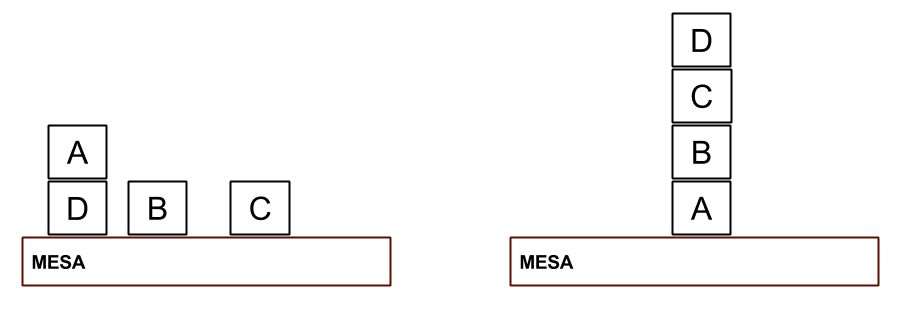
\includegraphics[width=10cm]{figures/blocos.png}
  \caption{Exemplo de estado inicial e final para o Mundo dos Blocos}
  \label{fig:blocos}
\end{figure}

Com o domínio do mundo dos blocos, fizemos trinta e cinco testes com um número de blocos de quatro até dezessete. Para cada número de blocos do problema, tínhamos três diferentes configurações de estado inicial e final.

\subsubsection{Resultados}\label{problemas:blocos:resultados}

%Grafico para time - Mundo dos blocos
\begin{figure}[H]
\centering
\begin{tikzpicture}
  \begin{axis}[
      only marks, xtick=data, xticklabels 
from table={plot/timeBlocos2.dat}{Problema},
      xticklabel style={rotate=90},
      axis lines=left,
      xlabel={Problemas do Mundo dos Blocos},
      xlabel style={at={(0.5,-0.05)}},
      ylabel={Tempo de Execução em milissegundos $log_{10}$},
      enlarge x limits={abs={0.0001*\pgfplotbarwidth}},
      legend style={at={(0.5,-0.20)},anchor=north,legend columns=1},
      height=9cm, width=15cm]

      \addplot table [x expr=\coordindex, y=H0]{plot/timeBlocos2.dat};
      \addplot table [x expr=\coordindex,
      y=GraphPlanHeuristic]{plot/timeBlocos2.dat};
      \addplot table [x expr=\coordindex, 
      y=GraphPlanHeuristicOpt]{plot/timeBlocos2.dat};
      \addplot table [x expr=\coordindex, 
      y=HSP_AddHeuristic]{plot/timeBlocos2.dat};
      \addplot table [x expr=\coordindex, 
      y=HSP_MaxHeuristic]{plot/timeBlocos2.dat};

  \legend{H0, Graph Plan, Graph Plan Otimo, HSP ADD, HSP MAX}
  \end{axis}
\end{tikzpicture}
\caption{Tempo de Execução - Mundo dos blocos}
\label{fig:timeBlocos}
\end{figure}
%%%%%%%%%%%%

Quanto ao tempo de execução, vemos na figura \ref{fig:timeBlocos} que a heurística HSPAdd foi a que melhor produziu resultados, conseguindo resolver problemas mais difíceis. Já o GraphPlan foi o que teve o pior comportamento: foi o que mais demorou para devolver uma solução e o que resolveu a menor quantidade de problemas.

%Grafico para nos Visitados - Mundo dos blocos
\begin{figure}[H]
\centering
\begin{tikzpicture}
  \begin{axis}[
      only marks, xtick=data, xticklabels 
from table={plot/visitadosBlocos.dat}{Problema},
      xticklabel style={rotate=90},
      axis lines=left,
      xlabel={Problemas do Mundo dos Blocos},
      xlabel style={at={(0.5,-0.05)}},
      ylabel={Número de nós Visitados ($log_{10}$)},
      enlarge x limits={abs={0.0001*\pgfplotbarwidth}},
      legend style={at={(0.5,-0.20)},anchor=north,legend columns=1},
      height=9cm, width=15cm]

      \addplot table [x expr=\coordindex, y=H0]{plot/visitadosBlocos.dat};
      \addplot table [x expr=\coordindex,
      y=GraphPlanHeuristic]{plot/visitadosBlocos.dat};
      \addplot table [x expr=\coordindex, 
      y=GraphPlanHeuristicOpt]{plot/visitadosBlocos.dat};
      \addplot table [x expr=\coordindex, 
      y=HSP_AddHeuristic]{plot/visitadosBlocos.dat};
      \addplot table [x expr=\coordindex, 
      y=HSP_MaxHeuristic]{plot/visitadosBlocos.dat};
  \legend{H0, Graph Plan, Graph Plan Otimo, HSP ADD, HSP MAX}
  \end{axis}
\end{tikzpicture}
\caption{Nós Visitados - Mundo dos blocos}
\label{fig:visitadosBlocos}
\end{figure}

A figura \ref{fig:visitadosBlocos} mostra que a heurística HSPAdd visitou o menor número de nós para todas os problemas. Já a heurística H0 foi a que visitou o maior número de nós. Isso já era esperado porque a H0 produz uma busca em largura no grafo.

%Nos gerados e visitados Blocos
\begin{table}[H]
\begin{tabular}{l|l|l|l|l|l|l|l|l|l|l|}
\cline{2-11}
                            & \multicolumn{2}{c|}{H0} & \multicolumn{2}{c|}{\begin{tabular}[c]{@{}c@{}}Graph \\ Plan\end{tabular}} & \multicolumn{2}{c|}{\begin{tabular}[c]{@{}c@{}}Graph \\ Plan \\ Optimo\end{tabular}} & \multicolumn{2}{c|}{\begin{tabular}[c]{@{}c@{}}HSP \\ ADD\end{tabular}} & \multicolumn{2}{c|}{\begin{tabular}[c]{@{}c@{}}HSP \\ MAX\end{tabular}} \\ \hline
\multicolumn{1}{|l|}{Prob.} & Visit.     & Ger.       & Visit.                               & Ger.                                & Visit.                                    & Ger.                                     & Visit.                              & Ger.                              & Visit.                              & Ger.                              \\ \hline
\multicolumn{1}{|l|}{4-0}   & 125        & 257        & 37                                   & 55                                  & 33                                        & 48                                       & 19                                  & 25                                & 38                                  & 53                                \\ \hline
\multicolumn{1}{|l|}{4-1}   & 110        & 224        & 30                                   & 46                                  & 27                                        & 42                                       & 22                                  & 32                                & 36                                  & 52                                \\ \hline
\multicolumn{1}{|l|}{4-2}   & 109        & 220        & 29                                   & 43                                  & 19                                        & 27                                       & 18                                  & 24                                & 32                                  & 44                                \\ \hline
\multicolumn{1}{|l|}{5-0}   & 732        & 1647       & 182                                  & 308                                 & 130                                       & 209                                      & 61                                  & 83                                & 119                                 & 167                               \\ \hline
\multicolumn{1}{|l|}{5-1}   & 796        & 1867       & 165                                  & 280                                 & 100                                       & 163                                      & 38                                  & 50                                & 110                                 & 152                               \\ \hline
\multicolumn{1}{|l|}{5-2}   & 866        & 2044       & 601                                  & 1198                                & 350                                       & 648                                      & 60                                  & 81                                & 124                                 & 173                               \\ \hline
\multicolumn{1}{|l|}{6-0}   & 4372       & 10363      & 335                                  & 590                                 & 123                                       & 187                                      & 110                                 & 145                               & 157                                 & 239                               \\ \hline
\multicolumn{1}{|l|}{6-1}   & 6601       & 17108      & 5411                                 & 11830                               & 373                                       & 585                                      & 69                                  & 91                                & 282                                 & 374                               \\ \hline
\multicolumn{1}{|l|}{6-2}   & 7057       & 18473      & 4822                                 & 10137                               & 3143                                      & 6555                                     & 105                                 & 137                               & 409                                 & 568                               \\ \hline
\multicolumn{1}{|l|}{7-0}   & 54696      & 149861     & 28867                                & 57943                               & 3394                                      & 5865                                     & 122                                 & 159                               & 2035                                & 3154                              \\ \hline
\multicolumn{1}{|l|}{7-1}   & 65990      & 185278     & 55370                                & 133602                              & 25511                                     & 55594                                    & 216                                 & 277                               & 2213                                & 3557                              \\ \hline
\multicolumn{1}{|l|}{7-2}   & 64676      & 181625     & 38891                                & 82129                               & 21759                                     & 45321                                    & 127                                 & 183                               & 2808                                & 4358                              \\ \hline
\multicolumn{1}{|l|}{8-0}   & 641879     & 1915788    & -1                                   & -1                                  & 43151                                     & 78721                                    & 210                                 & 256                               & 11498                               & 19168                             \\ \hline
\end{tabular}
\caption{Nós Visitados e Gerados - Mundos dos Blocos}
\label{tab:nosBlocos}
\end{table}

A tabela \ref{fig:custoBlocos} apresenta os nós visitados e gerados para todas as heurísticas usadas. Valores -1 significam que o problema não terminou de ser resolvido. Ressaltamos que a otimização feita no GraphPlan resultou em menor número de nós visitados e gerados. Porém, o HSPAdd foi a heurística que apresentou melhores resultados nesses quesitos.

%Grafico para custo - Mundo dos blocos
\begin{figure}[H]
\centering
\begin{tikzpicture}
  \begin{axis}[
      only marks, xtick=data, xticklabels 
from table={plot/custoBlocos.dat}{Problema},
      xticklabel style={rotate=90},
      axis lines=left,
      xlabel={Problemas do Mundo dos blocos},
      xlabel style={at={(0.5,-0.05)}},
      ylabel={Custo da Solução},
      enlarge x limits={abs={0.0001*\pgfplotbarwidth}},
      legend style={at={(0.5,-0.20)},anchor=north,legend columns=1},
      height=9cm, width=15cm]

      \addplot table [x expr=\coordindex, y=H0]{plot/custoBlocos.dat};
      \addplot table [x expr=\coordindex,
      y=GraphPlanHeuristic]{plot/custoBlocos.dat};
      \addplot table [x expr=\coordindex, 
      y=GraphPlanHeuristicOpt]{plot/custoBlocos.dat};
      \addplot table [x expr=\coordindex, 
      y=HSP_AddHeuristic]{plot/custoBlocos.dat};
      \addplot table [x expr=\coordindex, 
      y=HSP_MaxHeuristic]{plot/custoBlocos.dat};
  \legend{H0, Graph Plan, Graph Plan Otimo, HSP ADD, HSP MAX}
  \end{axis}
\end{tikzpicture}
\caption{Custo da Solução - Mundo dos blocos}
\label{fig:custoBlocos}
\end{figure}

Por fim, em relação ao custo da solução, a figura \ref{fig:custoBlocos} mostra que, para as primeiras instâncias do problema, as heurísticas empatam. Já para instâncias maiores, o GraphPlan otimizado e a H0 apresentam as soluções com menor custo.

\subsection{Robôs}\label{problemas:robos}

O problema dos robôs consiste de um robô, $x$ caixas e $y$ salas. Inicialmente, cada caixa está em uma determinada sala e, como meta do problema, as caixas devem permanecer na mesma sala ou serem transportadas até outra sala.

O robô é o agente responsável por transportar as caixas de uma sala para outra. Ele pode carregar até duas caixas (uma em cada braço), movê-las para outra sala e em seguida descarregá-las. As salas desse domínio são posicionadas de tal forma que, se o robô estiver em uma sala $x_i$, pode se mover para qualquer uma das outras salas que o problema possui. A Figura \ref{fig:salas} mostra o exemplo de um estado desse domínio. Neste exemplo, o problema possui quatro salas (Room 1, Room 2, Room 3 e Room 4) e quatro caixas (B1, B2, B3 e B4).

\begin{figure}[H]%[htb]
  \centering
  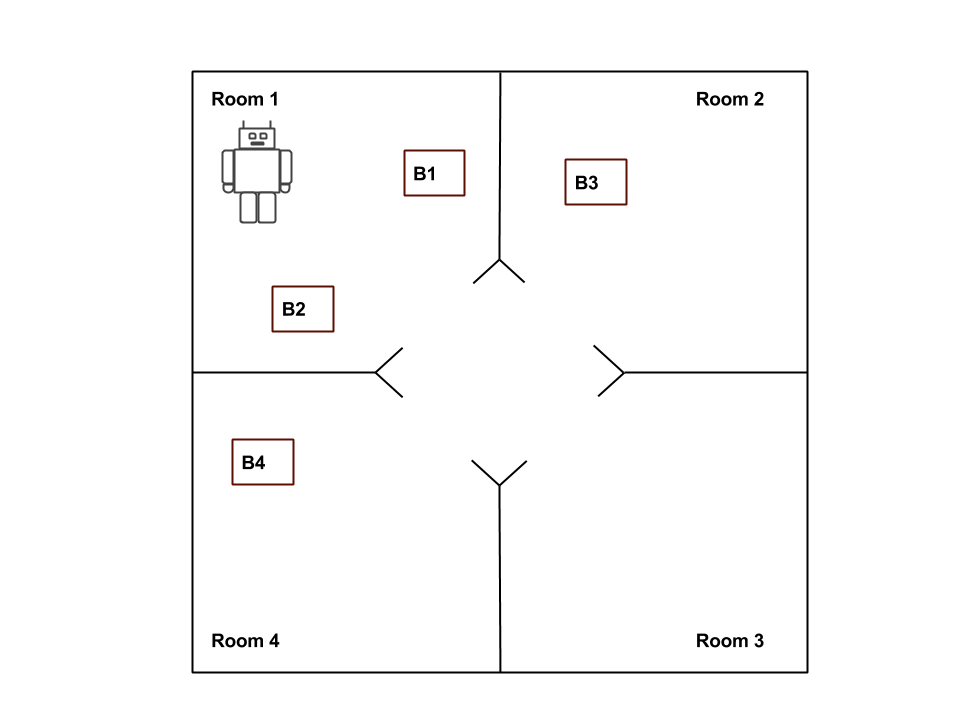
\includegraphics[width=10cm]{figures/salas.png}
  \caption{Estado para problema dos Robôs}
  \label{fig:salas}
\end{figure}

Usando o domínio dos robôs, rodamos experimentos para vinte diferentes estados iniciais e finais. Nos dez primeiros, tínhamos duas salas e número de caixas de um até dez (para cada novo teste, adicionávamos uma caixa). Todas as caixas estavam inicialmente em uma sala (Room 1) e como estado final deveriam estar na outra sala (Room 2).

Nos outros dez problemas, o número de salas também aumentou conforme aumentamos o número de caixas. Nestes problemas, cada caixa era posicionada inicialmente de tal forma que no estado final deveria estar na sala ao lado. Por exemplo, uma caixa inicialmente na sala 2 tem como meta estar na sala 3, uma caixa na sala 4 deve ir para 5 e assim por diante.

\subsubsection{Resultados}\label{problemas:robos:resultados}

%Grafico para time - Robos
\begin{figure}[H]
\centering
\begin{tikzpicture}
  \begin{axis}[
      only marks, xtick=data, xticklabels 
from table={plot/timeRobos2.dat}{Problema},
      xticklabel style={rotate=90},
      axis lines=left,
      xlabel={Problemas dos Robôs},
      xlabel style={at={(0.5,-0.1)}},
      ylabel={Tempo de Execução em milissegundos $log_{10}$},
      enlarge x limits={abs={0.0001*\pgfplotbarwidth}},
      legend style={at={(0.85,0.4)},anchor=north,legend columns=1},
      height=9cm, width=15cm]

      \addplot table [x expr=\coordindex, y=H0]{plot/timeRobos2.dat};
      \addplot table [x expr=\coordindex,
      y=GraphPlanHeuristic]{plot/timeRobos2.dat};
      \addplot table [x expr=\coordindex, 
      y=GraphPlanHeuristicOpt]{plot/timeRobos2.dat};
      \addplot table [x expr=\coordindex, 
      y=HSP_AddHeuristic]{plot/timeRobos2.dat};
      \addplot table [x expr=\coordindex, 
      y=HSP_MaxHeuristic]{plot/timeRobos2.dat};
  \legend{H0, Graph Plan, Graph Plan Otimo, HSP ADD, HSP MAX}
  \end{axis}
\end{tikzpicture}
\caption{Tempo de Execução - Problema dos Robôs}
\label{fig:tempoRobos}
\end{figure}




%Grafico para custo - Robos
\begin{figure}[H]
\centering
\begin{tikzpicture}
  \begin{axis}[
      only marks, xtick=data, xticklabels 
from table={plot/custoRobos.dat}{Problema},
      xticklabel style={rotate=90},
      axis lines=left,
      xlabel={Problemas dos Robôs},
      xlabel style={at={(0.5,-0.1)}},
      ylabel={Custo da Solução},
      enlarge x limits={abs={0.0001*\pgfplotbarwidth}},
      legend style={at={(0.85,0.4)},anchor=north,legend columns=1},
      height=9cm, width=15cm]

      \addplot table [x expr=\coordindex, y=H0]{plot/custoRobos.dat};
      \addplot table [x expr=\coordindex,
      y=GraphPlanHeuristic]{plot/custoRobos.dat};
      \addplot table [x expr=\coordindex, 
      y=GraphPlanHeuristicOpt]{plot/custoRobos.dat};
      \addplot table [x expr=\coordindex, 
      y=HSP_AddHeuristic]{plot/custoRobos.dat};
      \addplot table [x expr=\coordindex, 
      y=HSP_MaxHeuristic]{plot/custoRobos.dat};
  \legend{H0, Graph Plan, Graph Plan Otimo, HSP ADD, HSP MAX}
  \end{axis}
\end{tikzpicture}
\caption{Custo da Solução - Problema dos Robôs}
\label{fig:custoRobos}
\end{figure}


%Nos gerados e visitados Robos
\begin{table}[H]
\begin{tabular}{l|l|l|l|l|l|l|l|l|l|l|}
\cline{2-11}
                            & \multicolumn{2}{c|}{H0} & \multicolumn{2}{c|}{\begin{tabular}[c]{@{}c@{}}Graph \\ Plan\end{tabular}} & \multicolumn{2}{c|}{\begin{tabular}[c]{@{}c@{}}Graph \\ Plan \\ Optimo\end{tabular}} & \multicolumn{2}{c|}{\begin{tabular}[c]{@{}c@{}}HSP \\ ADD\end{tabular}} & \multicolumn{2}{c|}{\begin{tabular}[c]{@{}c@{}}HSP \\ MAX\end{tabular}} \\ \hline
\multicolumn{1}{|l|}{Prob.} & Visit.     & Ger.       & Visit                               & Ger.                                 & Visit.                                    & Ger.                                     & Visit.                              & Ger.                              & Visit.                              & Ger.                              \\ \hline
\multicolumn{1}{|l|}{2}     & 28         & 70         & 11                                  & 16                                   & 26                                        & 53                                       & 17                                  & 34                                & 17                                  & 34                                \\ \hline
\multicolumn{1}{|l|}{3}     & 297        & 1082       & 22                                  & 34                                   & 154                                       & 354                                      & 53                                  & 98                                & 53                                  & 98                                \\ \hline
\multicolumn{1}{|l|}{4}     & 3816       & 17549      & 37                                  & 58                                   & 928                                       & 2170                                     & 119                                 & 245                               & 119                                 & 245                               \\ \hline
\multicolumn{1}{|l|}{5}     & 58523      & 322124     & 56                                  & 88                                   & 4485                                      & 10168                                    & 269                                 & 618                               & 269                                 & 618                               \\ \hline
\multicolumn{1}{|l|}{6}     & -1         & -1         & 79                                  & 124                                  & 26019                                     & 56571                                    & 353                                 & 953                               & 353                                 & 953                               \\ \hline
\multicolumn{1}{|l|}{7}     & -1         & -1         & 106                                 & 166                                  & -1                                        & -1                                       & 537                                 & 1580                              & 537                                 & 1580                              \\ \hline
\multicolumn{1}{|l|}{8}     & -1         & -1         & -1                                  & -1                                   & -1                                        & -1                                       & -1                                  & -1                                & -1                                  & -1                                \\ \hline
\multicolumn{1}{|l|}{9}     & -1         & -1         & 172                                 & 268                                  & -1                                        & -1                                       & 1061                                & 3708                              & 1061                                & 3708                              \\ \hline
\multicolumn{1}{|l|}{10}    & -1         & -1         & 211                                 & 328                                  & -1                                        & -1                                       & 1438                                & 5389                              & 1438                                & 5389                              \\ \hline
\multicolumn{1}{|l|}{2B2R}  & 27         & 66         & 23                                  & 41                                   & 27                                        & 62                                       & 18                                  & 29                                & 18                                  & 29                                \\ \hline
\multicolumn{1}{|l|}{3B2R}  & 87         & 272        & 51                                  & 87                                   & 87                                        & 272                                      & 42                                  & 76                                & 42                                  & 76                                \\ \hline
\multicolumn{1}{|l|}{4B2R}  & 255        & 882        & 192                                 & 486                                  & 255                                       & 870                                      & 69                                  & 130                               & 69                                  & 130                               \\ \hline
\multicolumn{1}{|l|}{5B2R}  & 703        & 2612       & 603                                 & 1857                                 & 703                                       & 2612                                     & 158                                 & 319                               & 158                                 & 319                               \\ \hline
\multicolumn{1}{|l|}{6B2R}  & 1855       & 7214       & 1710                                & 5876                                 & 1855                                      & 7194                                     & 229                                 & 475                               & 229                                 & 475                               \\ \hline
\multicolumn{1}{|l|}{7B2R}  & 4735       & 19056      & 4537                                & 16707                                & 4735                                      & 19056                                    & 746                                 & 1666                              & 746                                 & 1666                              \\ \hline
\multicolumn{1}{|l|}{8B2R}  & 11775      & 48618      & 11516                               & 44450                                & 11775                                     & 48590                                    & 1017                                & 2290                              & 1017                                & 2290                              \\ \hline
\multicolumn{1}{|l|}{9B2R}  & 28671      & 120812     & 28343                               & 113157                               & 28671                                     & 120812                                   & 3890                                & 9305                              & 3890                                & 9305                              \\ \hline
\multicolumn{1}{|l|}{10B2R} & 68607      & 293862     & 68202                               & 279264                               & 68607                                     & 293826                                   & 5081                                & 12101                             & 5081                                & 12101                             \\ \hline
\end{tabular}
\caption{Nós Visitados e Gerados - Problema dos Robôs}
\label{tab:nosRobos}
\end{table}

Na figura \ref{fig:tempoRobos} podemos observar que a heurística GraphPlan foi a que produziu tempos menores seguida de HSPAdd, conseguindo resolver problemas mais difíceis, para as instâncias onde o robô tem que deixar as caixas em outros quartos. Já o HSPMax, e o H0 foi os que tiveram o pior comportamento: foi o que mais demorou para devolver uma solução e o que resolveu a menor quantidade de problemas.

Na segunda parte do problema, onde os robôs tem de deixar as caixas no quarto 2, o GraphPlan produziu os piores resultados, em parte devido ao tempo de computação da heurística. O H0, produziu os melhores resultados precisamente por isso.

A tabela \ref{fig:custoBlocos} apresenta o custo das soluções encontradas.
O custo mínimo vem dado pelo uso da heurística H0 que é admissível.
O GraphPlan e o HSPAdd são heurísticas não admissíveis e as soluções encontradas tem um custo maior.

\subsection{Satélites}\label{problemas:satelites}

Neste domínio, há um conjunto de satélites equipados com diferentes instrumentos, os quais com características diferentes em relação a calibração dos alvos, produção de dados e consumo de energia. Os satélites coletam dados e os mandam para uma estação base.

O objetivo é adquirir imagens desejadas da forma mais eficiente possível, dividindo as tarefas de observação entre os satélites baseado nas capacidades de seus instrumentos.

Para este domínio, fizemos testes com vinte problemas diferentes. Neles, variamos a quantidade de satélites, seus instrumentos e suas configurações e também o número de fenômenos, estrelas, planetas e imagens. Este domínio é o mais complexo dos três que testamos pela variabilidade de objetos, ações e predicados.

\subsubsection{Resultados}\label{problemas:satelites:resultados}

Por ser muito complexo, o domínio dos satélites foi o que apresentou menos resultados como podemos ver na figura \ref{fig:timeSatellite}.
Neste domínio vemos que a heurística H0 somente consegue resolver o primeiro problema, e que HSP Add é quem apresenta melhores resultados, conseguindo resolver mais problemas que o resto de heurísticas.

Uma das causas do baixo desempenho das heurísticas GraphPlan é o alto número de ações que precisam ser tratadas na heurística e que precisariam ser ordenadas resultando em um custo computacional mais alto.

Na seção \ref{analise} poderão ser vistos melhores resultados neste domínio obtidos modificando o peso da função heurística (WA*).


%Time Satellite
\begin{figure}[H]
\centering
\begin{tikzpicture}
  \begin{axis}[
      only marks, xtick=data, xticklabels 
from table={plot/timeSatellite.dat}{Problema},
      xticklabel style={rotate=0},
      axis lines=left,
      xlabel={Problemas dos Satélites},
      ylabel={Tempo de Execução em milissegundos $log_{10}$},
      enlarge x limits={abs={0.0001*\pgfplotbarwidth}},
      legend style={at={(0.85,0.4)},anchor=north,legend columns=1},
      height=9cm, width=9cm]

      \addplot table [x expr=\coordindex, y=H0]{plot/timeSatellite.dat};
      \addplot table [x expr=\coordindex,
      y=GraphPlanHeuristic]{plot/timeSatellite.dat};
      \addplot table [x expr=\coordindex, 
      y=GraphPlanHeuristicOpt]{plot/timeSatellite.dat};
      \addplot table [x expr=\coordindex, 
      y=HSP_AddHeuristic]{plot/timeSatellite.dat};
      \addplot table [x expr=\coordindex, 
      y=HSP_MaxHeuristic]{plot/timeSatellite.dat};
  \legend{H0, Graph Plan, Graph Plan Otimo, HSP ADD, HSP MAX}
  \end{axis}
\end{tikzpicture}
\caption{Tempo de Execução - Problema dos Satélites}
\label{fig:timeSatellite}
\end{figure}


%Custo Satellite
\begin{figure}[H]
\centering
\begin{tikzpicture}
  \begin{axis}[
      only marks, xtick=data, xticklabels 
from table={plot/custoSatellite.dat}{Problema},
      xticklabel style={rotate=0},
      axis lines=left,
      xlabel={Problemas dos Satélites},
      ylabel={Custo da Solução},
      enlarge x limits={abs={0.0001*\pgfplotbarwidth}},
      legend style={at={(0.85,0.4)},anchor=north,legend columns=1},
      height=9cm, width=9cm]

      \addplot table [x expr=\coordindex, y=H0]{plot/custoSatellite.dat};
      \addplot table [x expr=\coordindex,
      y=GraphPlanHeuristic]{plot/custoSatellite.dat};
      \addplot table [x expr=\coordindex, 
      y=GraphPlanHeuristicOpt]{plot/custoSatellite.dat};
      \addplot table [x expr=\coordindex, 
      y=HSP_AddHeuristic]{plot/custoSatellite.dat};
      \addplot table [x expr=\coordindex, 
      y=HSP_MaxHeuristic]{plot/custoSatellite.dat};
  \legend{H0, Graph Plan, Graph Plan Otimo, HSP ADD, HSP MAX}
  \end{axis}
\end{tikzpicture}
\caption{Custo da Solução - Problema dos Satélites}
\label{fig:timeSatellite}
\end{figure}



\section{Análise do W}\label{analise}

Para a maior parte dos problemas, a variação do W não teve impacto significativo em sua resolução. Porém, para o domínio dos satélites, a diferença foi notável. A tabela \ref{analisew} mostra os tempos de execução para os problemas resolvidos do domínio dos satélites, com W=2 e W=5. A heurística usada foi a HSPAdd. Não houve muita diferença entre o tempo de resposta entre eles porém o resultado mais surpreendente é que nenhuma das outras heurísticas conseguiu terminar as instancias a partir da 7. Isso se deve ao fato de que, com o W maior, o plano vai mais diretamente para a meta. Por fim, vale ressaltar que a instância 18 do problema foi resolvida por provavelmente ter uma configuração mais simples.

\begin{table}[H]
\begin{tabular}{|l|l|l|}
\hline
Problema & \multicolumn{1}{c|}{W=2} & W=5        \\ \hline
1        & 66.44                    & 89.6       \\ \hline
2        & 403.7                    & 647.47     \\ \hline
3        & 1101.91                  & 789.21     \\ \hline
4        & 4445.59                  & 4750       \\ \hline
6        & 9818.14                  & 10287.3    \\ \hline
7        & 47314.89                 & 54180.04   \\ \hline
8        & 102525.41                & 105250.48  \\ \hline
9        & 315038.23                & 330873.44  \\ \hline
10       & 192070.33                & 196693.99  \\ \hline
18       & 1031454.12               & 1096534.54 \\ \hline
\end{tabular}
\caption{Tempo de Execução para W=2 e 5 HSP ADD - Problema dos Satélites}
\label{analisew}
\end{table}








%%%%%%%%%%%%%%%%%%%%%%%%%%%%%%%%%%%%%%%%%%%%%%%%%%%%%%

\section{Conclusões}\label{conclusao}
Os resultados mostram que na maioria dos domínios, usar uma heurística informativa é melhor que usar uma heurística nada informativa (H0), mesmo que seja uma não admissível. 
Somente no domínio do robô a heurística H0 pode ficar com bons resultados, por causa da estrutura do plano solução.

Mas os resultados não foram tão conclusivos como desejaríamos no caso da heurística do GraphPlan, por causa das estruturas de dados usadas.
Nos artigos estudados, os resultados do HSP são um pouco piores dos da heurística do GraphPlan.
Nossa implementação usa uma estrutura de dados que favorece às heurísticas de tipo HSP, e pode penalizar algumas das implementações com GraphPlan.
Mesmo tendo implementado a heurística otimizada como indicado nos artigos, ela mesmo pode ficar bem pior que o GraphPlan normal, devido a algumas operações que no pseudo-código ficam implícitas e no nosso código tivemos que implementar fazendo varreduras de vetores e outras estruturas que consomem mais tempo.






%%%%%%%%%%%%%%%%%%%%%%%%%%%%%%%%%%%%%%%%%%%%%%%%%%%%%%
\bibliographystyle{apalike}	% Tipo do formato da bibliografia
\bibliography{bibliografia}

\end{document}
